\documentclass[openany]{article}
\usepackage{times}
%\usepackage{mtpro2}
\usepackage{amsmath, amsthm, amssymb, calrsfs, wasysym, verbatim, bbm, bm, color, graphics, geometry,enumitem,tikz,pgfplots,dsfont, listings}
\usepackage{xcolor}
\usepackage[colorlinks=true, linkcolor = black!40!blue,
urlcolor  = black!40!red,
citecolor = blue,
anchorcolor = blue]{hyperref}
\frenchspacing
\setlength{\parindent}{0pt}

\title{Probability Theory for EOR (EBP014B05)\\
version: 2021-08-02}
\date{ Fall 2021}
\author{Lingwei Kong}
%\pagestyle{empty}


% % % % % % % % % % % % % % % % % % % % % % % % % %
\usepackage{tikz}
\usetikzlibrary{calc,trees,positioning,arrows,chains,shapes.geometric,%
	decorations.pathreplacing,decorations.pathmorphing,shapes,%
	matrix,shapes.symbols}

\tikzset{
	>=stealth',
	punktchain/.style={
		rectangle, 
		rounded corners, 
		% fill=black!10,
		draw=black, very thick,
		text width=11em, 
		minimum height=0em, 
%		text centered, 
		on chain},
	line/.style={draw, thick, <-},
	element/.style={
		tape,
		top color=white,
		bottom color=blue!50!black!60!,
		minimum width=8em,
		draw=blue!40!black!90, very thick,
		text width=10em, 
		minimum height=3.5em, 
		text centered, 
		on chain},
	every join/.style={->, thick,shorten >=1pt},
	decoration={brace},
	tuborg/.style={decorate},
	tubnode/.style={midway, right=2pt},
}
\usetikzlibrary{shapes,arrows}
\tikzstyle{small_block} = [circle, draw, fill=white!20, 
text width=0em, text centered, rounded corners, minimum height=0em]   
\begin{document}
\maketitle\thispagestyle{empty}
\textit{Welcome to the course Probability Theory for EOR - Edition 2021/2022. In
	this outline, you can find information on the organization of the course. This course syllabus is based on the one by Dr. T. Boot, who had previously taught this course. Many thanks for his help.\\~\\
	 Furthermore, there were limitations over the on-campus activities (e.g., capacity limit over the class size) when designing this course. We had to adapt to the online teaching framework at that moment. There is no room left for re-designing and re-scheduling for block 1B, \textbf{therefore you will notice that most activities are still online except the tutorials and the exams}. Still, we may make some changes accordingly in the future.} 
 \tableofcontents
 
 
 \newpage
\section{Description}
Economic outcomes are inherently uncertain: a factory does not know for
sure when a certain machine breaks down, a government does not know
for sure whether lowering taxes will increase consumption, you do not know
for sure whether studying econometrics will improve your future wealth and
well-being.\\~\\
To have a meaningful conversation about the probability of
certain events, we need to specify what we mean by the term probability. This makes probability theory a central building block for studying econometrics and operations research.\\~\\
In this course, we develop the (mathematical) language needed to discuss probabilities properly. We will, for example, talk about sample spaces (set
of possible outcomes), events (a subset of possible outcomes), probability distributions (a coherent way to assign a probability to an event). We hope you understand that a random variable is simply a specific function with underlying sample space and a probability function. 

A crucial
the concept is that of a conditional probability: how do possibilities change
when new information comes in?\\~\\
The formal course objectives are the following. Upon completion of the
course you will be able to:
\begin{enumerate}
	\item Quantify uncertainty using a coherent framework for probability.
	\item Understand the concept of a conditional probability and use conditional
	probability as a problem solving tool.
	\item Understand the concept of a random variable and derive properties of
	well-known discrete and continuous random variables.
	\item Calculate the expected value of discrete and continuous random variables.
	\item Simulate and visualize the outcomes of chance experiments on your
	computer.
\end{enumerate}
This course would require mathematical concepts covered in Math I, and this course will be followed by Probability Distributions in block 2.1 (using
the same book) and Estimation and Testing in block 2.2. 
%\let\cleardoublepage\clearpage
\section{Course Organization}
 ~\\
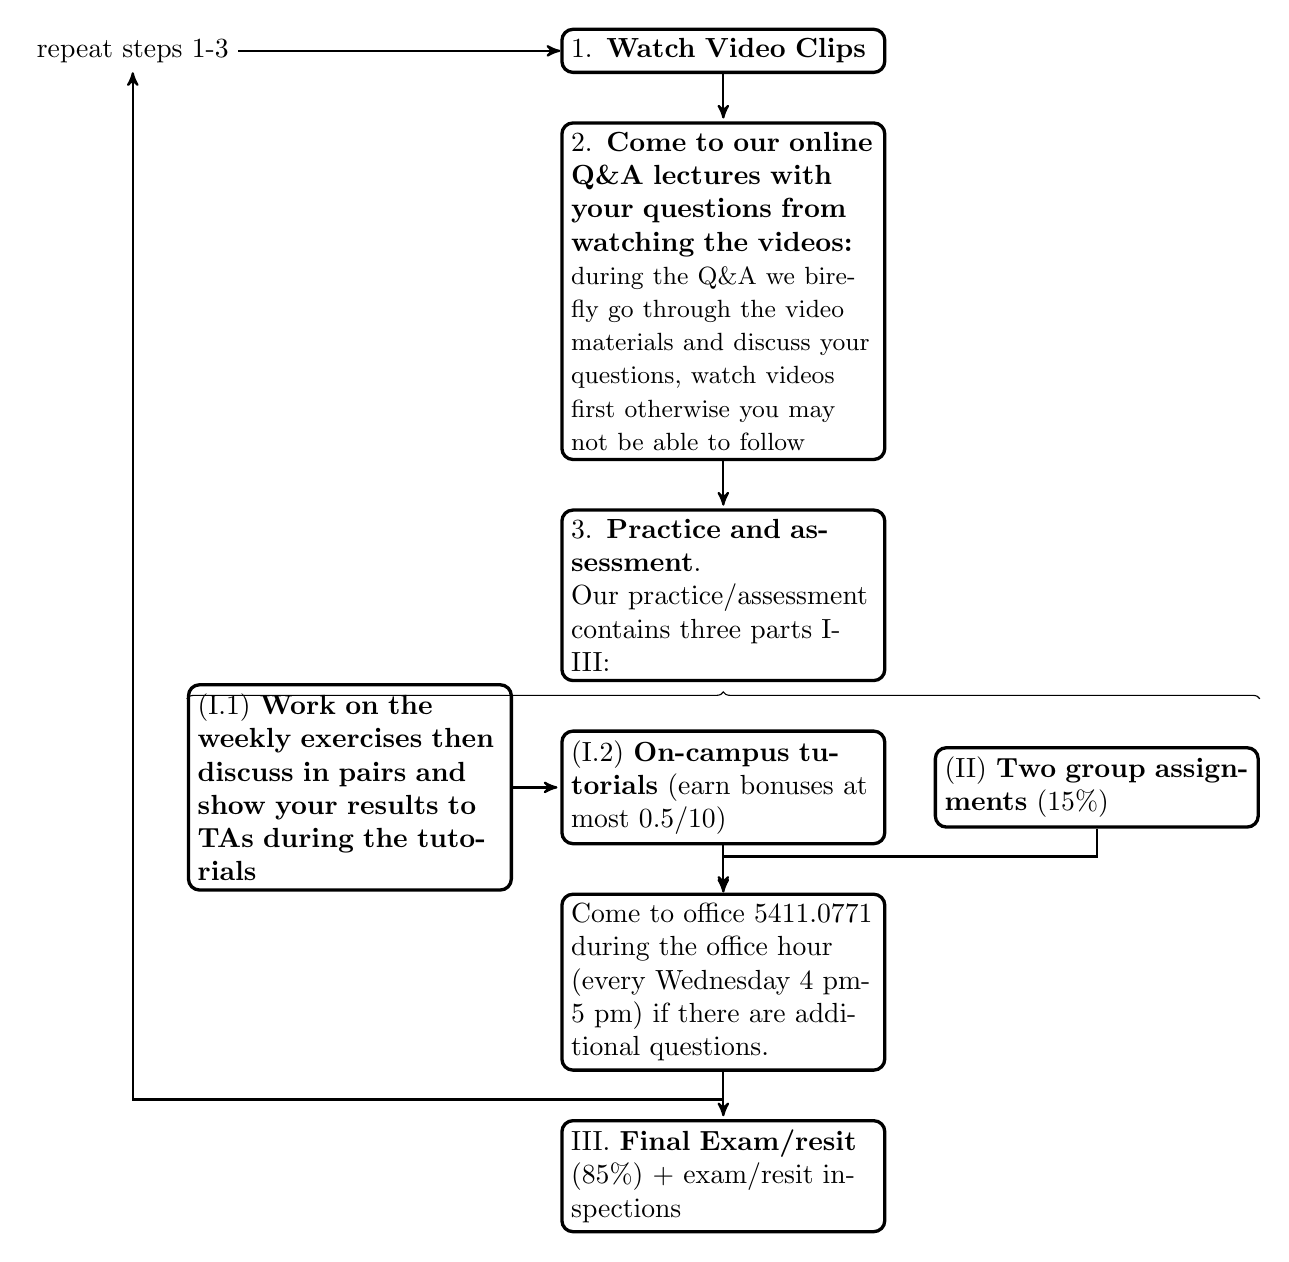
\begin{tikzpicture}
	[node distance=.6cm,
	start chain=going below,]
	\node[punktchain, join] (intro) {1. \textbf{Watch Video Clips}}; 
	\node[punktchain, join] (investeringer)      {2. \textbf{Come to our online Q\&A lectures with your questions from watching the videos:} \small during the Q\&A we birefly go through the video materials and discuss your questions, watch videos first otherwise you may not be able to follow};
	
	\node[punktchain, join] (intro2) {3.  \textbf{\textbf{Practice and assessment}}. \\Our practice/assessment contains three parts I-III:};
%	\node[punktchain, join] (perfekt) {Det perfekte kapitalmarked};
%	\node[punktchain, join, ] (emperi) {Emperi};
	\node (asym) [punktchain ]  {(I.2) \textbf{On-campus tutorials} (earn bonuses at most 0.5/10)};
	\begin{scope}[start branch=venstre,
		%We need to redefine the join-style to have the -> turn out right
		every join/.style={->, thick, shorten <=1pt}, ]
		\node[punktchain, on chain=going left, join=by {<-}]
		(risiko) { (I.1) \textbf{Work on the weekly exercises then discuss in pairs and show your results to TAs during the tutorials}};
	\end{scope}
	\begin{scope}[start branch=hoejre,]
		\node (finans) [punktchain, on chain=going right] {(II) \textbf{Two group assignments} (15\%)};
	\end{scope}
	\node[punktchain, join,] (disk) {Come to office 5411.0771 during the office hour (every Wednesday 4 pm-5 pm) if there are additional questions.};
	\node[punktchain, join,] (makro) {III. \textbf{Final Exam/resit} (85\%) + exam/resit inspections};
	
%	\node[punktchain, join] (konk) {Konklusion};
	% Now that we have finished the main figure let us add some "after-drawings"
	%% First, let us connect (finans) with (disk). We want it to have
	%% square corners.
	\draw[|-,-|,->, thick,] (finans.south) |-+(0,-1em)-| (disk.north);
	 \node [left of=intro, node distance=7.5cm] (update) {repeat steps 1-3};
	\draw[|-,-|,->, thick,] (disk.south) |-+(0,-1em)-| (update); 
	\path [line] (intro) -- (update);
%	\draw[|-,-|,->, thick,] (update.east) |-+(0,-1em)-| (intro.west); 
%	 \path [line] (disk) -| (intro);
%	\draw  (disk.south) to[out=-20,in=-70] (intro.west)
	% Now, let us add some braches. 
	%% No. 1
	\draw[tuborg] let
	\p1=(risiko.west), \p2=(finans.east) in
	($(\x1,\y1+3.2em)$) -- ($(\x2,\y2+3.2 em)$) node[above, midway]  {~\\~\\ };
	%% No. 2
%	\draw[tuborg, decoration={brace}] let \p1=(disk.north), \p2=(makro.south) in
%	($(2, \y1)$) -- ($(2, \y2)$) node[tubnode] {Analyse};
	%% No. 3
%	\draw[tuborg, decoration={brace}] let \p1=(perfekt.north), \p2=(emperi.south) in
%	($(2, \y1)$) -- ($(2, \y2)$) node[tubnode] {Problemfelt};
\end{tikzpicture}~\\ \clearpage
\subsection{Material}
The course is based on Chapter 1 – 6 of Introduction to Probability, Second Edition by J.K. Blitzstein and J. Hwang and published by CRC Press. \\~\\
A digital version of the book is available for free via \href{https://projects.iq.harvard.edu/stat110/home}{this webpage}, which
is filled with useful resources (for example, there are YouTube videos with
lectures by the author). If you can, I recommend getting a physical copy of
the book (as this makes studying easier, and you are going to need it for the course Probability Distribution as well). \\~\\
We also store other teaching materials on a public \href{https://github.com/}{Github} repository:\\ \href{https://github.com/lingwei-kong/RuG_ProbabilityTheory_for_EOR_LKong}{https://github.com/lingwei-kong/RuG\_ProbabilityTheory\_for\_EOR\_LKong}

GitHub is a handy tool for collaborating with your teams, and here is one starting guide for your Github -- "Hello, World.":
\href{https://guides.github.com/activities/hello-world/}{https://guides.github.com/activities/hello-world/} \\
It is not compulsory to use GitHub.
\subsection{Videos and Q\&A lectures}
\textbf{Watch the videos (knowledge clips) before coming to our Q\&A lectures}. We have one Q\&A lecture each week. On Wednesday from 10:00 – 11:00. These lectures consist of roughly 30
minutes of a brief explanation of this week’s topics (so it is a quick summary, and you will need to watch videos first to follow) and then ask your questions (see Section \ref{section question} for all the places you may leave your questions) from watching the videos along with these brief summaries. These Q\&A lectures are not recorded, so ask whatever questions you have.\\~\\ 
\textbf{Other materials for preparing for the lectures:} A schedule showing the subjects discussed in each lecture is provided on Nestor, under Course Documents. Use the textbook, slides, especially exercises each week, to facilitate your studies. \\~\\
\textbf{Aim} The aim of the videos is to provide a comprehensive discussion of new
theoretical concepts. And we review briefly during our online sessions where you can ask any questions raised up while watching the videos. For the exam, all material from the book as listed in the Subject Overview is relevant (also, the material not discussed in
the lectures).\\~\\
\textbf{Slides} Slides used during the videos will be made available simultaneously along with the videos. 

\subsection{Weekly exercises and on campus tutorials}
There is one on-campus tutorial session each week. The group composition can be found on Nestor. Join the tutorial for discussions and BONUSES!\\~\\
\textbf{I.} {The first 45 minutes} of the tutorial will be used to discuss
relevant exercises. You can discuss in pairs with your classmates (i.e., discuss with the one sitting next to you, and I highly recommend that you discuss with different classmates in each tutorial). \textbf{Show your discussed results (written solutions and some feedback from your peers) to your teaching assistants (TAs) during the first 45 minutes or the break if you could not finish, this is how you earn your bonuses}. You benefit most from the tutorials if you have gone over the exercises prior to the tutorial.
\begin{itemize}
	\item The feedback for your results will be made by four categories: 1 (for the presence of the tutorials); 5 (partial solutions); 10 (sufficient results). 
	\item For every 7 points you earn during the tutorials, you would get 0.1 extra bonus added to your final marks, and you can earn at most 0.5 bonuses. 
\end{itemize}
\textbf{II.} {The remaining 45 minutes,} TAs will present the solutions, and feel free to ask questions. \\~\\
\begin{tabular}{llll} 
	Group & Day & Time & TA \\
	\hline Group 1 & Thursday & 11:00-13:00 & Joost Doornbos\\
	Group 2 & Thursday & 11:00-13:00 & Sander van Beek\\ 
	
	Group 3 & Thursday & 13:00-15:00 & Sander van Beek\\
	Group 4 & Thursday & 13:00-15:00 & Karlijn Zwiggelaar\\
	Group 5 & Friday & 11:00-13:00 & Quinten Huisman\\
	
	Group 6 & Friday & 11:00-13:00 & Karlijn Zwiggelaar \\
	Group 7 & Friday & 13:00-15:00 & Quinten Huisman\\
	Group 8 & Friday & 13:00-15:00 & Joost Doornbos\\
\end{tabular}~\\~\\~\\
\textbf{Exercises and solutions} The exercises are listed in the schedule, which
can be found on Nestor, under Course Information. Solutions to questions
that are not discussed during the tutorials will be made available at the end
of the week.

\subsection{Group assignments}
There will be two assignments that are due on Friday
19:00 in week 3 and 6. The assignments will consist of some theoretical
exercises mixed with some basic coding to verify the results. The assignments
are to be made in groups of 2 students from the same tutorial group. \\~\\
Deadline
to enroll in these groups is Friday November 19 at 19:00. You can
enroll by clicking Assignments in the main menu of the Nestor Course and
then clicking Enroll here.\\~\\
Students that are re-taking the course also have to participate in
the assignments.\\~\\
Please contact the course coordinator at least three days before the deadline if 
you want to switch groups between assignments and everyone involved agrees or
if you encounter problems in collaborating with your fellow group member.  

\subsection{On campus exam/resit}
\textbf{Open book exam/resit}: you can bring any printed out/hand-written materials and the textbook. It is, however under no circumstances allowed to
communicate (either online or offline) with anyone else during the exam.
Any suspected case of fraud will be sent to the Board of Examiners.\\~\\
\textbf{Extra time } In case you are granted additional time by the Board of Examiners, this will be added after the official end time of the exam.

\subsection{Locations for on-campus activities}
Please check the Rooster for the exact schedules and locations of our on-campus activities:\\ \href{https://rooster.rug.nl/#/en/current/schedule/course-EBP014B05}{https://rooster.rug.nl/\#/en/current/schedule/course-EBP014B05}.
\subsection{Grading}
Denote: 
\begin{itemize}
	\item $A_i\in [0,15]$: Grade on Assignment i, where $i$ = 1; 2.	
	\item $T_i\in \{1, 5, 10\}$: Grade on Tutorials i, where $i$ = 1; 2; ...;7.	
	\item $E\in [0,10]$: Exam/resit grade.  
	\item $C\in [0,10]$: Course Grade.
	\item $P$: Progress Grade (the grade stored in your system).
\end{itemize}
If an assignment is missing, you will receive a 0 on that assignment. Note
that if you retake the course, you have to hand in the assignments as well!
If $E > 5$ (so you score a 5 or higher on the exam/resit), then
{\scriptsize $$C=\left\{ \begin{matrix}
E & \textit{if}~E\leq 5 \\
\min \left\{ 0.85*E + 0.15* \textit{round}\left( 10*\frac{1}{2} \frac{1}{15} (\sum_{i=1}^{2}A_i)  \right)+ \min \left\{0.1* \textit{round}\left( \frac{1}{7} (\sum_{i=1}^{7}T_i)  \right), 0.5\right\}, 10 \right\} & \textit{if} ~E> 5
\end{matrix} \right. $$}~\\
 You pass the course if $C\geq 5.5$ and the Progress grade $P = \textit{round}(C)$.\\~\\ Finally, if you hand in two assignments, but you do not take part
 in the exam/resit, you will receive E = 1, and the corresponding grade P = 1 will
 be entered in Progress.
\section{Contact information}
The course is taught by Lingwei Kong, who can be reached at
\href{mailto:l.kong@rug.nl}{l.kong@rug.nl} and 5411.0771. Hans Ligtenberg \href{mailto:j.w.ligtenberg@rug.nl}{j.w.ligtenberg@rug.nl} would assistant our course.\\~\\
Extra office hours at 5411.0771: every Wednesday 4pm-5pm.\\~\\
Contact info for our TAs:\\~\\
\begin{tabular}{llll} 
		\hline	\hline\\
	Karlijn Zwiggelaar& \href{mailto:k.a.h.zwiggelaar@student.rug.nl}{k.a.h.zwiggelaar@student.rug.nl} \\
	Joost Doornbos& \href{mailto:joostdoornbos01@gmail.com}{joostdoornbos01@gmail.com} \\
	Quinten Huisman&  \href{mailto:q.n.huisman@student.rug.nl}{q.n.huisman@student.rug.nl} \\
	Sander van Beek& \href{mailto:s.g.h.van.beek@student.rug.nl}{s.g.h.van.beek@student.rug.nl} \\	\hline
\end{tabular}
 
\section{Question on the course/material/...}\label{section question}
 If you have questions on the course organization, the material, exercises,
 assignments, exam, then you can pose these:
 \begin{enumerate}
 	\item During our Q\&A lectures: directly unmute yourself, or click the raise-hand button or type the chatbox. 
 	\item During the tutorials: discuss with your TAs.
 	\item Via the Nestor Discussion Board. Also, use this to help each other! Recommended!
 	\item Via email (only for questions that are not relevant for other students).
 \end{enumerate}
\section{General remarks}
Find a buddy. Given the course's hybrid nature (online and on-campus), one of the main challenges is motivating yourself to keep up with the material. It helps enormously work with someone and schedule specific hours in a week where
you work on the course.\\~\\
Start working in week 1. Don't underestimate the material. The first week might look like things you had in high school, but previous years have
shown that for example, How to count is one of the most difficult subjects(and the course, in general, being one of the most difficult courses of the first
year).
\end{document}
